\documentclass[11pt,a4paper,titlepage]{report}
\usepackage[utf8]{inputenc}
\usepackage{graphicx}
\usepackage{listings}
\usepackage[T1]{fontenc}
\usepackage{lmodern}
\usepackage{hyperref}
\usepackage{xcolor}
\usepackage{pdflscape}

\newcommand{\code}[1]{{\ttfamily\small #1}}
\lstset{
  basicstyle=\ttfamily\small,
  frame=lines,
  columns=fullflexible,
  breaklines=true,
  captionpos=b,
  commentstyle=\color{white!50!black},
  escapeinside={\%*}{*)},
  keywordstyle=\color{blue},
  stringstyle=\color{green!50!black}
}
\lstdefinestyle{Antlr}{
  moredelim=[s][\color{green!50!black}]{'}{'},
  moredelim=*[s][\color{black}]{options}{\}},
  commentstyle={\color{white!50!black}},
  morecomment=[l]{//},
  alsoletter={:,|,;},
  morekeywords={:,|,;,grammar},
  keywordstyle={\color{blue}},
}

\newcommand{\name}{Open Transport Language Deluxe }
\newcommand{\shortname}{\textsc{otld} }

\title{\Huge Open Transport Language Deluxe \\ \vspace{5mm} \Large Final project for Compiler Construction \\ University of Twente}

\author{
Martijn Bruning \\
\small s1363999
\and Jan-Jelle Kester \\
\small s1337718
}

\date{\today}

\begin{document}

\maketitle

\tableofcontents

\chapter{Introduction}

Open Transport Language Deluxe (OTLD) is a programming language designed for the Compiler Construction course at the University of Twente.

\section{The language}

The language resembles Pascal, but the terminology is based on the ideas of the game `Open Transport Tycoon Deluxe'.
An OTLD program, a \emph{city}, defines all game elements first. The executable code of a program reads like delivery note.

The resemblance of the language with the OpenTTD game allows us to show the meaning of statements with examples from the game. Eventually, we think it would be nice if an OTLD program could be compiled to an OpenTTD save file, but that is out of the scope of the project for now.

\section{This report}

This report describes the OTLD language, including some design considerations and implementation details. The described implementation details include the implementation of the front end compiler, intermediate language and Java bytecode back end compiler.

\chapter{Language features}

This chapter provides a quick description of the main features of Open Transport Language Deluxe (OTLD).

OTLD supports boolean, integer and character types.
All these types can be used as arguments for functions, read from input and written to output.

\begin{itemize}
\item \textbf{Basic expression language}
	\begin{itemize}
	\item Variables using \emph{wagons}
	\item Single operator expressions using \emph{transports} and predefined \emph{factories}
		\begin{itemize}
		\item Unary minus (integers)
		\item Unary not (booleans)
		\item Multiplication, division, modulo division (integers)
		\item Addition, subtraction (integers)
		\item Equality \texttt{<}, \texttt{<=}, \texttt{>=}, \texttt{>} (integers)
		\item Equality \texttt{==}, \texttt{!=} (all types)
		\item (Logical) and, or (integers, booleans)
		\end{itemize}
	\end{itemize}
\item \textbf{\texttt{if} and \texttt{while}}
	\begin{itemize}
	\item \texttt{if} / \texttt{else} blocks for branches through \emph{signals}
	\item \texttt{while} loops through \emph{waypoints}
	\end{itemize}
\item \textbf{Procedures and functions}
	\begin{itemize}
	\item Non-nested, Java-like functions though \emph{factories}
	\item Read from standard input through \emph{ceo}
	\item Write to standard output through \emph{journal}
	\end{itemize}
\end{itemize}

\chapter{Problems and solutions}

\section{Java Virtual Machine}
\label{subj:asm}

We decided to build our language for the Java Virtual Machine.
This meant that we had to get to know Java bytecode.
We found that the way bytecode works is easy to understand, however, writing a correct Java class file is a lot trickier.

To tackle this problem we used the ASM library from ObjectWeb (\url{http://asm.ow2.org/}).
This library provides a class for programmatically writing Java classes using a visitor pattern.
This simplified bytecode generation a whole lot since it takes care of the structure of the file, including class, field an method definitions.
We still had to use Java opcodes to build the method bodies, but the frames are computed automatically by the library.

\chapter{Language specification}

\section{Layout of a program}

Defining a program in \shortname is like defining a program in Pascal, only in \shortname you are defining a \emph{city}. A city can be defined with the command \code{City <name>;}, where \code{<name>} is replaced with the name of the program.

\subsection{City blocks}

A city consists of a number of blocks, each containing integral parts of the program. Each block starts with the statement \code{Begin <block>;} and ends with \code{End <block>;}. Multiple blocks of the same type are supported, the contents of any block other than the first will be treated as it was appended to the first block of the type.

\begin{itemize}
\item \code{industry}: This block should contain all factories of the city.
\item \code{depot}: This block should contain all wagons and trains.
\item \code{track}: This block should contain all signals and waypoints.
\item \code{company}: This block should contain the program itself.
\end{itemize}

\subsubsection*{Example}

\begin{lstlisting}
Begin depot;
	Wagon w accepts coal;
	Train t accepts 6 steel;
End depot;
\end{lstlisting}

\section{Basic expressions}

\subsection{Constants}

Constants can not be declared as such. However, they can be used in the program, for example in assignments. The list below contains the available types with a regex showing the valid inputs.

Strings cannot be used in variables, but are only included for in- and outputs.

\begin{itemize}
\item Integer: \verb=-?(0|[1-9][0-9]*)=
\item Boolean: \verb=red|green= (where \verb|red| is false and \verb|green| is true)
\item Character: \verb='[a-zA-Z0-9]'=
\item String: \verb="~["]*(""~["]*)*"=
\end{itemize}

\subsection{Variable declarations}

Variables in \shortname are called \emph{wagons}. Wagons are statically typed. The type should be set on declaration.
A wagon can be declared with the statement \code{Wagon <id> accepts <type>;} where \code{<id>} is a unique identifier for the wagon and \code{<type>} is the type of the wagon. Variables can only be declared in the \code{depot} city block.

Booleans can also be stored in a \emph{signal}. The declaration and assignment of signals is different from wagons. A signal can be declared with the statement \code{Signal <id> is <color>;} where \code{<color>} is either \code{red} or \code{green}. Signals are used with conditionals. Signals can only be declared in the \code{track} city block.

\subsubsection*{Example}

\begin{lstlisting}
Wagon w1 accepts int;
Wagon w2 accepts boolean;
Signal s is green;
\end{lstlisting}

\subsection{Assignment}

A constant value or a value from another variable can be assigned to a variable.

To assign a constant to a variable use the statement \code{Load <const> into wagon <id>;} where \code{<const>} is the constant and \code{<id>} is the identifier for the wagon.

To copy the value of an existing wagon into another wagon use \code{Transfer wagon <id> to wagon <id>;}. The term `transfer' does not mean that the source wagon will be empty -- it remains untouched.

\subsubsection*{Example}

\begin{lstlisting}
Load 10 into wagon w1;
Transfer wagon w1 into wagon w2;
\end{lstlisting}

\subsection{Arithmetic operations}

There are two unary operations with each a special syntax:

\begin{itemize}
\item Unary minus: Inverts a wagon. \\ \code{Turn wagon <id> around;}
\item Not (for signals): Inverts a signal. \\ \code{Switch signal <id>;}
\end{itemize}

The other operations use the statement \code{Transport <id>, <id> to factory <op> and fully load <id>;}. The first to occurances of \code{<id>} are the left- and righthand variables for the operation, the third \code{<id>} is the destination wagon. The operation \code{<op>} can be any of the following:

\begin{itemize}
\item Addition: \code{add}
\item Subtraction: \code{subtract}
\item Multiplication: \code{multiply}
\item Division: \code{divide}
\item Modulo division: \code{modulo}
\item Less than: \code{complt}
\item Greater than: \code{compgt}
\item Less than or equal: \code{complte}
\item Greater than or equal: \code{compgte}
\item Equal: \code{compeq}
\item Logical and: \code{and}
\item Logical or: \code{or}
\end{itemize}

The operations that return a boolean can be used in two ways; either as mentioned above or with the statement \code{Transport <id>, <id> to factory <op> and set signal <id>;} to store the boolean in a signal.

\subsubsection*{Example}

\begin{lstlisting}
Transport w1, w2 to factory multiply and fully load w1;
Transport w1, w2 to factory complt and set signal s2;
Transport s1, s2 to factory and and set signal s1;
\end{lstlisting}

\section{Block statments}

\subsection{Conditionals (if/else)}

Conditional statements are based on signals. A conditional statement starts with \code{Approach signal <id>;} where \code{<id>} is the signal that indicates which path to choose. Code under \code{Case green;} is executed when the signal is green, code under \code{Case red;} is executed when the signal is red. The statement ends with \code{Pass signal;}.

The \code{Case} statements are not required, these just function as the start points for each block. The code under these statements is executed up until another \code{Case} statement or \code{Pass signal}. Multiple case statements for the same boolean value are allowed, however, the code of a second statement will just be appended to the code from the first.

\subsubsection*{Example}

\begin{lstlisting}
Approach signal s;
	Case red:
		Write "Train delayed" to journal;
Pass signal;
\end{lstlisting}
% TODO this has changed

\subsection{Loops (while)}

In \shortname \emph{circles} can be used for loops. Before defining the loop itself, the loop condition (\emph{waypoint}) needs to be defined. A waypoint can be defined with \code{Waypoint <id>;}. A waypoint behaves exactly the same way as a signal, but with one difference. It is possible to programmatically define the value of the waypoint every time it is accessed. To do this, add a waypoint block directly after the waypoint (\code{Begin waypoint;} and \code{End waypoint;}). Code in this waypoint block should write a boolean value to the identifier of the waypoint. Waypoints can only be declared in the \code{track} city block.

The code that should be executed in each iteration should be in a circle block starting with \code{Begin circle <id>;} and ending with \code{End circle;} where \code{<id>} is the identifier of the waypoint. To break out of a circle the statement \code{Stop;} can be used.

\subsubsection*{Example}

\begin{lstlisting}
Waypoint p;
Begin waypoint;
	Transport i, length to factory complt and set signal p;
End waypoint;

Begin circle p;
	Write "This is executed a single time" to journal;
	Stop;
	Write "This is not executed" to journal;
End circle;
\end{lstlisting}
% TODO this has changed

\subsection{Functions}

Functions are represented as \emph{factories}. Factories can be defined in the \code{industry} city block using the statement \code{Factory <id> accepts <type>[, <type>]* produces <type>;}, where \code{<id>} is the name of the factory and \code{<type>} is one of the supported variable types. This statement should be directly followed by a \code{production} block for the body of the function. This block should always end with \code{Final product <var>;}, which returns \code{<var>}. Returns are only allowed at this spot. The arguments can be accessed in the function body using \code{platformX} as variable name, where \code{X} is the 1-indexed argument index.

A function can be called similarly to an arithmetic operation with the \code{Transport <id>, <id> to factory <op> and fully load <id>;} statement where \code{<op>} is the factory name.

\subsubsection*{Example}

\begin{lstlisting}
Factory isZero accepts int produces boolean;
Begin production;
	Load 0 into wagon zero;
	Transport platform1, zero to factory eq and fully load temp;
	Final product temp;
End production;

Transport w1 to factory half and set signal s1;
\end{lstlisting}


\chapter{Implementation details}

We chose for an approach using an intermediate representation.
While an intermediate representation is not strictly necessary for our language, we found that it simplified development.
The intermediate representation allowed us to work on the front end and back end compiler at the same time, without having to discuss many things, which sped up the development process.

The central part of our application, which ties everything together, is the \code{Main} class.

\section{Front end compiler}

% Visitor

\section{Intermediate representation}

The intermediate representation allows us to represent a program as a tree of Java objects.
This helps on the front end side by making the visitor easier as in most cases a visitor method only has to create a new object and add it to the right parent.
Intermediate classes do type checking where possible.

The intermediate representation can be used with other source and target languages.
However, it has been designed for OTLD as source languages, so it might miss some or many features which are necessary to completely support other source languages.

Target languages are supported through the abstract \code{Compiler} class, which provides a structure for visitor-based back end compilers.

Details on the different classes can be found in the Javadoc of the \code{intermediate} package. The class diagram of this package has been included on page \pageref{fig:class_diagram__intermediate}.

\begin{figure}[p]
\centering
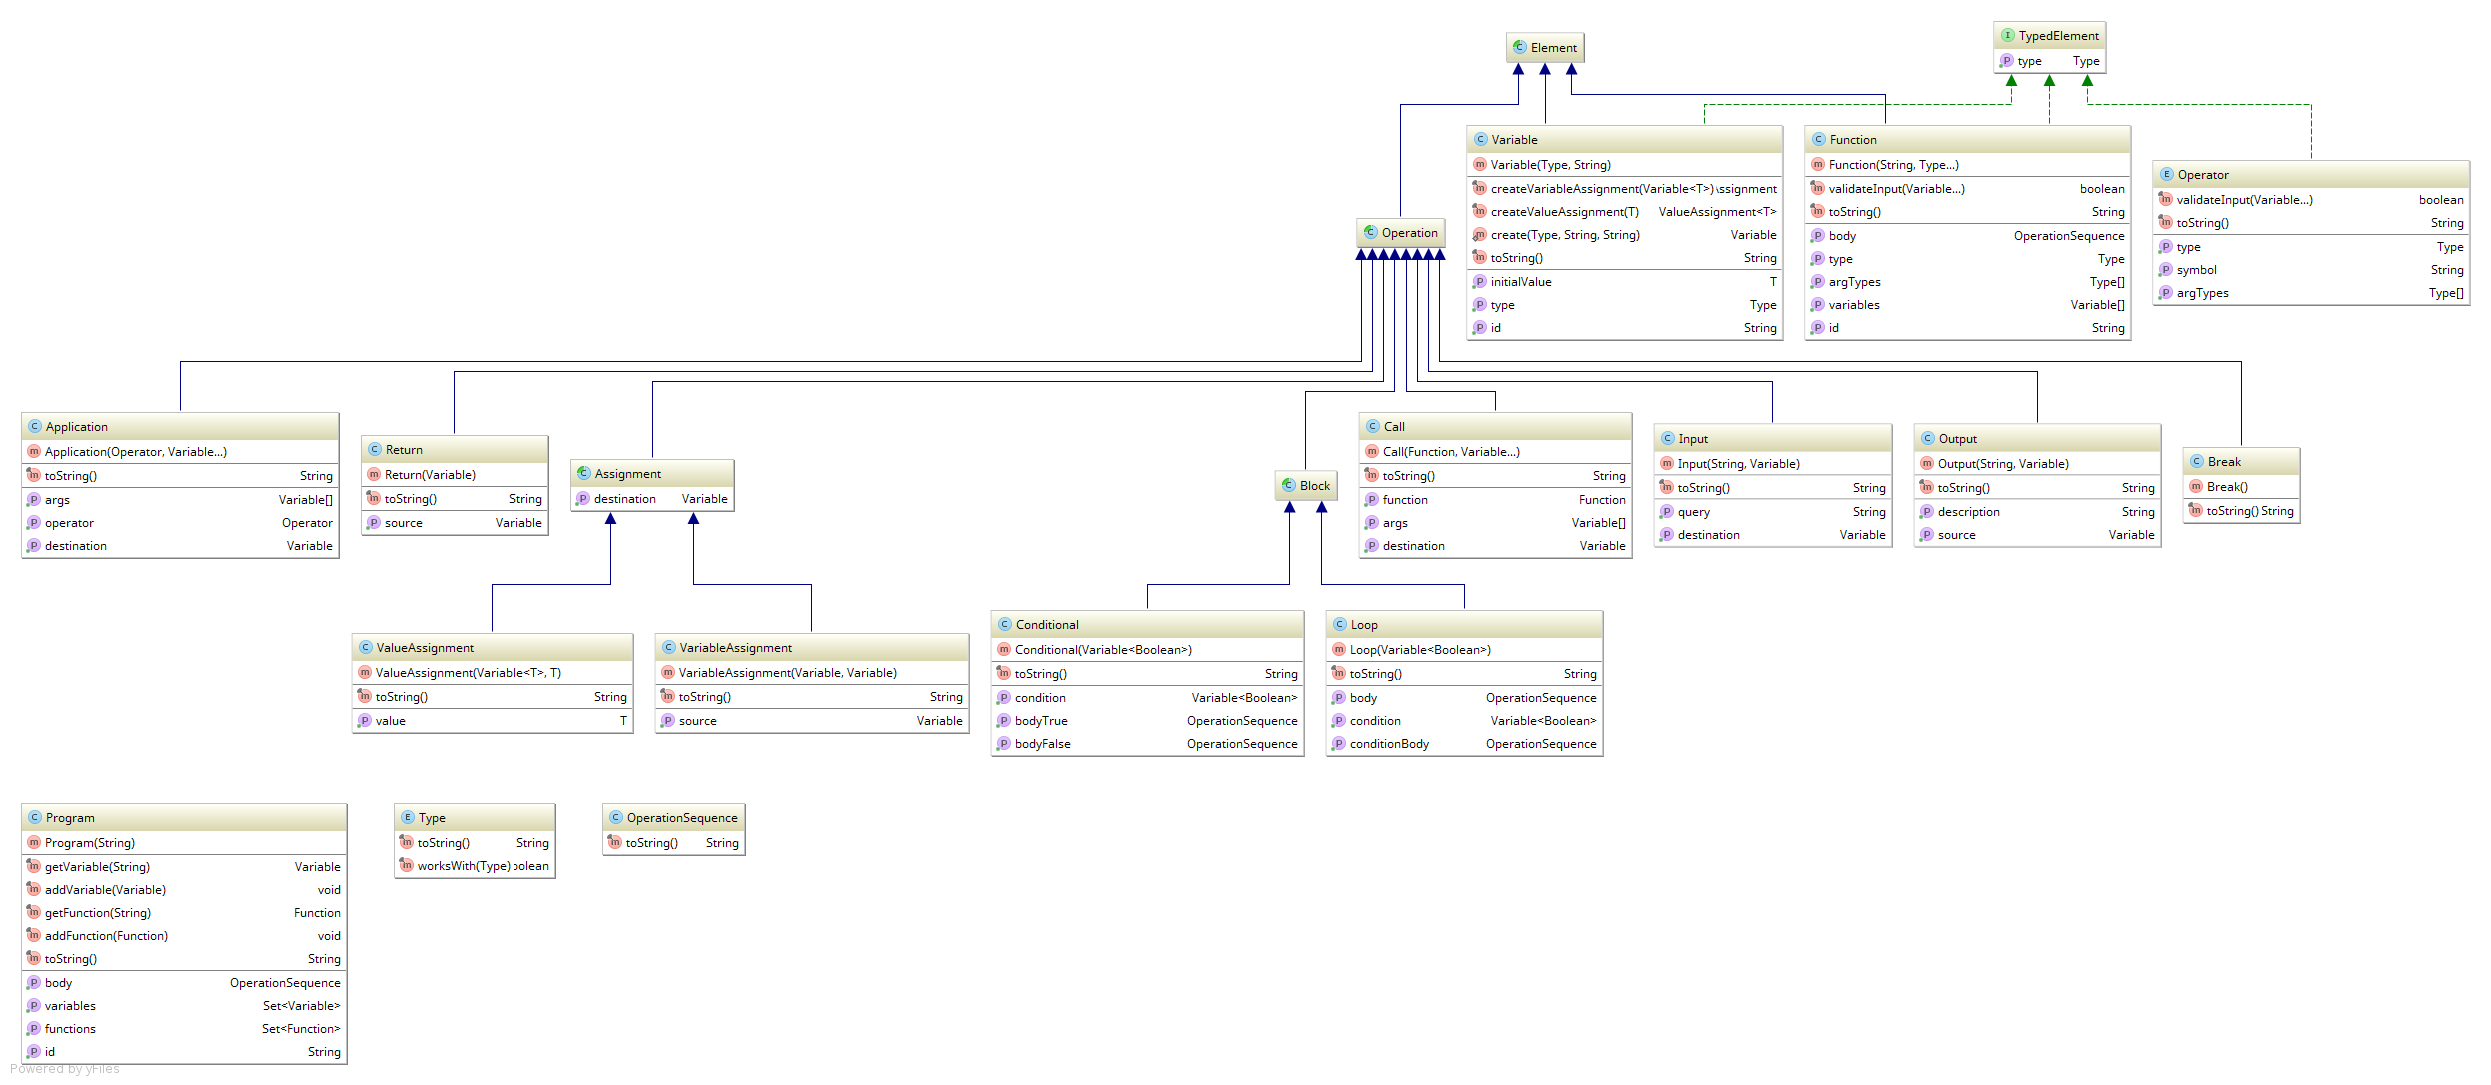
\includegraphics{Images/class_diagram__intermediate}
\caption{Class diagram for the intermedate representation}
\label{fig:class_diagram__intermediate}
\end{figure}

\section{Back end compiler}

The back end compiler is an implementation of the \code{Compiler} abstract class of the intermediate representation.
This means that it uses a visitor pattern to go through the tree of intermedate representation objects.
The back end compiler uses an ASM \code{ClassWriter} to create the program.
ASM is described in detail on page \pageref{subj:asm}.
The detailed description for each visitor method can be found in the Javadoc for the \code{jvm} package.

The back end compiler builds a Java class file from scratch.
The program code is put in the static main method, so the class file can be executed directly.
The class (and file) name correspond to the name of the program.
User-defined functions are added as public methods, and user-defined variables as public fields.

\chapter{Test plan}

The Open Transport Language Deluxe compiler consists of three parts.
We tested each part individually, while assuming that the other parts work as expected.
Additionally, we tested the whole compiler using a test program which features almost all possible operations.

We have used unit tests for the front end compiler and the intermediate representation.
The back end compiler does not feature many automated testing since there are no easy tools for automatically inspecting the resulting bytecode.
However, we wrote a unit test which compiles a program using all visitor methods on the back end compiler.
Furthermore, the ASM class writer calls are checked by ASM for abnormalities while compiling this program.
We also ran and inspected the resulting class file manually with \texttt{javap} and the IntelliJ decompiler.

\chapter{Conclusions}

We found the project a lot of fun to do.
This started with inventing our own language.
After having the idea to make a language inspired by Transport Tycoon Deluxe, coming up with a syntax required a lot of ingenuity since it was hard to come up with good analogies.
We also tried to make the language not too easy to use, since that would ruin part of the fun.
However, OTLD proved to be more usable than anticipated.

Writing an Antlr grammar and visitor was not too difficult for us after following the Vertalerbouw course.
However, the Java bytecode proved to be a good challenge.
Luckily, the Java VM is very well documented.
Also, the ASM library takes a lot of the difficult work out of our hands, like calculating frames, maximum stack and local variable sizes, besides just providing a good interface for writing Java class files.

We would have liked to put more time and effort into the project to improve our language, documentation and implementation.
However, other courses at the UT also required a lot of our time.
Therefore almost all of the work had to be done after July 6th, which put a bit of stress on our work.

In conclusion, we learned from working on this project, besides from it only being fun.
Although we would have liked to add more features, we are happy with the result.


\appendix

\chapter{Grammar}

% TODO
\begin{lstlisting}
\end{lstlisting}

\chapter{Tree walker}

% TODO
\begin{landscape}
\begin{lstlisting}[language=Java]
\end{lstlisting}
\end{landscape}

\chapter{Complete test program}
\label{chap:testprogram}

\begin{landscape}
\begin{lstlisting}
City Enschede;

/** Correctly working program, still need to think of something to do with char. */
Begin depot;
    Wagon a accepts int;
    Wagon b accepts boolean;
    Wagon c accepts char;
    Wagon d accepts int;
End depot;

Begin track;
    Signal s is red;
    Signal s2 is red;
    Signal s3 is green;

    Waypoint w;
    Begin waypoint;
        Write "Passed waypoint " w to journal;
    End waypoint;
End track;

Begin industry;
    Factory notLessThanOrEquals accepts int, int produces boolean;

    Begin production;
        Transport platform1, platform2 to factory complte and fully load platform3;
        Turn wagon platform3 around;

        Final product platform3;
    End production;
End industry;

Begin company;
    Ask control "a=?" about contents of a;
    Load 0 into wagon d;

    Transport a,d to factory compgt and fully load s;

    Approach signal s;
        Case green:
            Load 0 into wagon d;
        Case red:
            Stop;
        Case green:
            Switch signal s;
    Pass signal;

    Load 1 into wagon d;
    Load 'c' into wagon c;

    Transport a,a to factory notLessThanOrEquals and fully load b;
    Transport a,a to factory notLessThanOrEquals and set signal s2;

    Begin circle w;
        Transport a,d to factory subtract and fully load a;
        Transport a,d to factory notLessThanOrEquals and set signal w;
    End circle;

    Write "a=" a to journal;
    Write "b=" b to journal;
    Write "c=" c to journal;
    Write "d=" d to journal;

    Write "s=" s to journal;
    Write "s2=" s2 to journal;
    Write "s3=" s3 to journal;
End company;
\end{lstlisting}
\end{landscape}


\end{document}
